\section{Motivation}\label{chapter-01:section:motivation}

The machine learning community has seen unprecedented technological development in recent
years.
This thesis has been written at a time when computers have become able to generate unique
pictures in any possible art style, merely based on a small textual description.
Computers help to drive cars, help to control an airplane, help to navigate in an unfamiliar
city, and much more.
Incredibly, they are even capable of engaging in human-like conversations and providing
meaningful responses to factual questions.
Undoubtedly, these technological advances have transformed the ways in which we interact with
information and pursue knowledge.

These achievements would not have been possible without the tremendous computational
processing power that is available today.
Thousands of data centers around the world are devoted to the processing and analysis of
massive amounts of data, and seemingly generating intelligent decisions and artifacts through
these processes.
The question arises of how these large data-crunching processes, often collectively labeled
\ac{ai}, compare against ``intelligent'' reasoning in nature.
How does a bird learn to fly without employing simulations of wing aerodynamics?
How does a dog learn to recognize its owner without training on thousands of gigabytes of
photos captured from various angles and under different lighting conditions?
How does a human learn to speak Japanese without relying on dozens of high-end \acp{gpu} 
while exhaustively studying the entirety of available online content
written in Japanese?
These questions highlight the remarkable ability of biological systems to acquire
knowledge and make decisions without relying on large labeled and categorized data sets or
immense computational power stations.
There is clearly a difference in how natural and artificial systems acquire knowledge and
reason in an ``intelligent'' way.
%what we Despite the lack of large training data sets, we clearly recognize these biological systems as \textit{intelligent}.

\begin{figure}
  \centering
  \begin{tcolorbox}[width=\textwidth,arc=0pt,boxsep=0pt,left=0pt,right=0pt,top=0pt,bottom=0pt]
    
\includegraphics[width=\linewidth]{contents/01-introduction/figs/01-bird.png}
  \end{tcolorbox}
  \caption{An auto-generated image of ``a bird looking at a gigantic supercomputer, which consumes an enormous amount of energy, white background, 3:1 aspect ratio''.}
  \label{fig:intro:bird}
\end{figure}

\subsection{The Bayesian brain and the Free Energy principle}

It is well-documented that the human brain operates on approximately 20 watts of power
consumption \citep{raichle_appraising_2002} and it is estimated that the entire human body
consumes around 100 watts \citep{kovac_20_2010}.
In comparison, a typical halogen office light bulb consumes power ranging from 50 to 100
watts and a modern supercomputer power consumption can be as high as 60 megawatts\footnote{https://www.hpcwire.com/2021/09/08/how-argonne-is-preparing-for-exascale-in-2022/}.
Therefore, while engaging in real-time reasoning about how to maintain homeostasis through the
simultaneous processing of many sensory information sources, moving a heavy body through
space, and philosophizing about potential career perspectives, the human body consumes about the
same power as a stationary ceiling attachment.
Such an unparalleled level of energy efficiency is truly remarkable.

How does a body achieve this?
We do not know exactly, but there are some strong ideas. 
Amongst those ideas, the "Bayesian Brain" hypothesis suggests that the brain implements an approximate Bayesian
inference process to make sense of sensory information and perform cognitive tasks
\citep{doya_bayesian_2006}.
It suggests that the brain comprises a probabilistic model of its environment, continually
infers the likely causes of its sensorium, and updates its models on-the-fly when
prediction errors arise. 
But what is a probabilistic model and Bayesian inference?

\subsubsection{Probabilistic models and Bayesian inference}

A Bayesian inference process can be roughly described as \textit{learning about what we do not observe based on what we observe}.
In particular, the Bayesian approach provides a comprehensive mathematical framework for inference and statistical reasoning and describes a systematic way to update our prior beliefs and make informed decisions in the presence of uncertainty. 
Bayesian inference is often applied in reasoning together with \textit{probabilistic models}.
A probabilistic model $p(\bm{y}, \bm{s})$ is a structured representation of uncertainty and probabilistic relationships between observations $\bm{y}$ and hidden states $\bm{s}$. In this context \textit{``what we observe''} is $\bm{y}$ and \textit{``what we do not observe''} is $\bm{s}$.
Given a model $p(\bm{y}, \bm{s})$ and a set of new observations $\hat{\bm{y}}$, Bayesian inference uses Bayes rule to infer a posterior distribution $p(\bm{s}\vert\hat{\bm{y}})$, which represents our posterior beliefs about the hidden causes of these observations.
% \begin{equation}
%     \label{eq:intro:bayesrule}
%     \underbrace{p(\bm{s}\vert\bm{y})}_{\mathrm{posterior~beliefs}} \cdot \overbrace{\int p(\bm{y}\vert\bm{s})p(\bm{s})\mathrm{d}\bm{s}}^{\mathrm{evidence~}p(\bm{y})} = \underbrace{p(\bm{y}\vert\bm{s})}_{\mathrm{likelihood}}\cdot\overbrace{p(\bm{s})}^{\mathrm{prior~beliefs}}
% \end{equation}
\begin{figure}
  \centering
  \resizebox{1.0\textwidth}{!}{\begin{tikzpicture}[node distance=0.5mm, inner sep=0mm]
  %Nodes
  \node[] (eq) {$=$};
  \node[] (posterior) [left=of eq, yshift=0.25mm] {$p(\bm{s}\vert\hat{\bm{y}})$};
  \node[] (fractionleft) [right=of eq, yshift=0.25mm] {};
  \node[node distance=8mm] (fractioncenter) [right=of fractionleft] {};
  \node[node distance=8mm] (fractionright) [right=of fractioncenter] {};

  \path[-] (fractionleft.center) edge[] 
    node[pos=0.3, anchor=south, yshift=0.5mm](likelihood){$p(\hat{\bm{y}}\vert\bm{s})$}
    node[pos=0.8, anchor=south, yshift=0.5mm](prior){$p(\bm{s})$}
    node[pos=0.5, anchor=north, yshift=-0.5mm](evidence){$p(\hat{\bm{y}})$}
  (fractionright.center);

  \node[align=left] (posteriorcaption) [below=of posterior, yshift=-1mm, xshift=-17mm, align=left] {
  \begin{varwidth}{30mm}
      \small{Posterior}\\
      \tiny{probability distribution of the hidden states given observations} \\
      \tiny{\textit{(updated knowledge: how probable are hidden states given the observed data?)}}
    \end{varwidth}
  };

  \node[align=left] (likelihoodcaption) [above=of posterior, yshift=2mm, xshift=-15mm, align=left] {
  \begin{varwidth}{35mm}
      \small{Likelihood}\\
      \tiny{probability distribution for observed data, given hidden states. Since data is given, the likelihood is a function of states.} \\
      \tiny{\textit{(how ``likely'' are the states, given the data?)}}
    \end{varwidth}
  };

  \node[align=right] (priorcaption) [above=of posterior, yshift=0mm, xshift=46mm, align=right] {
  \begin{varwidth}{30mm}
      \small{Prior}\\
      \tiny{probability distribution of hidden states, before any observations} \\
      \tiny{\textit{(prior knowledge: how probable are the hidden states before observing any data?)}}
    \end{varwidth}
  };

  \node[align=right] (evidencecaption) [below=of posterior, yshift=-1mm, xshift=43mm, align=right] {
  \begin{varwidth}{35mm}
      \small{Evidence}\\
      \tiny{probability distribution of the observed data independently of the hidden states. Often interpreted  as a model score} \\
      \tiny{\textit{(how probable are these particular observations for this model?)}}
    \end{varwidth}
  };

  \draw (posteriorcaption.east) -| ([yshift=-1mm]posterior.south) node[pos=0.0, circle,fill=black,inner sep=0pt,minimum size=2pt]{} node[pos=1.0, circle,fill=black,inner sep=0pt,minimum size=2pt]{};

  \draw (likelihoodcaption.east) -| ([yshift=1mm]likelihood.north) node[pos=0.0, circle,fill=black,inner sep=0pt,minimum size=2pt]{} node[pos=1.0, circle,fill=black,inner sep=0pt,minimum size=2pt]{};

  \draw ([xshift=-1mm]priorcaption.west) -| ([yshift=1mm]prior.north) node[pos=0.0, circle,fill=black,inner sep=0pt,minimum size=2pt]{} node[pos=1.0, circle,fill=black,inner sep=0pt,minimum size=2pt]{};
  
  \draw ([xshift=-1mm]evidencecaption.west) -| ([yshift=-1mm]evidence.south) node[pos=0.0, circle,fill=black,inner sep=0pt,minimum size=2pt]{} node[pos=1.0, circle,fill=black,inner sep=0pt,minimum size=2pt]{};

\end{tikzpicture}}
  \caption{Schematic illustration of Bayes rule applied to the inference of hidden states $\bm{s}$ given actual observations $\hat{\bm{y}}$.}
  \label{fig:intro:bayesrule}
\end{figure}
In particular, in probabilistic models, the ``forward'' (generative) direction of the model describes how specific hidden states lead to observations and the ``backward'' (inference) direction relates to using the Bayes rule to derive the distribution over hidden states and update our prior beliefs for a given set of observations.
\begin{figure}
  \centering
  \resizebox{1.0\textwidth}{!}{\begin{tikzpicture}[]
  %Nodes
  \node[] (center) {};

  \node[box, fill=white] (model) {Probabilistic model~$p(\bm{y}, \bm{s})$};
  \node[box, minimum width=30mm] (prior) [left=of model]{Prior beliefs $p(\bm{s})$};
  \node[box, minimum width=30mm] (data) [right=of model]{Observations $p(\bm{y})$};

  \path[line, thick] (prior) edge[-] 
    node[pos=0.5](llinecenter){} 
    % node[pos=0.5, anchor=south](llinecentercaption){$\bm{s}$}
    (model);
  \path[line, thick] (model) edge[-] 
    node[pos=0.5](rlinecenter){} 
    % node[pos=0.5, anchor=south](rlinecentercaption){$\bm{y}$} 
    (data);

  \node[] (ltpivot) [above=of llinecenter, yshift=-5mm] {};
  \node[] (lbpivot) [below=of llinecenter, yshift=5mm] {};
  \node[] (rtpivot) [above=of rlinecenter, yshift=-5mm] {};
  \node[] (rbpivot) [below=of rlinecenter, yshift=5mm] {};

% $p(\bm{y}\vert\hat{\bm{s}}) = \frac{p(\hat{\bm{s}}\vert\bm{y})p(\bm{y})}{p(\hat{\bm{s}})}$
% $p(\bm{s}\vert\hat{\bm{y}}) = \frac{p(\hat{\bm{y}}\vert\bm{s})p(\bm{s})}{p(\hat{\bm{y}})}$

  \path[line, thick] (ltpivot) edge[-stealth] 
    node[pos=0.5, anchor=south]{Forward (generative)}
  (rtpivot);
  \path[line, thick] (rbpivot) edge[-stealth] 
    node[pos=0.5, anchor=north]{Backward (inference)}
  (lbpivot);
  
\end{tikzpicture}}
  \caption{Schematic illustration of an interaction between prior and actual observed information in a probabilistic model.
    In probabilistic models, the ``forward'' (generative) direction of the model describes how specific hidden states lead to observations and the ``backward'' (inference) direction relates to using the Bayes rule to derive the distribution over hidden states and update our prior beliefs for a given set of observations.
  }
  \label{fig:intro:bayesflow}
\end{figure}
The Bayesian approach finds extensive applications in signal processing \citep{bagautdinov_machine_2013}, healthcare \citep{lu_bayesian_2018}, forecasting \citep{berninger_bayesian_2020}, psychology \citep{wagenmakers_bayesian_2018}, and many more, and offers several advantages relative to non-Bayesian reasoning, such as
\begin{itemize}
    \item providing a coherent framework for incorporating prior knowledge and fusing information from
both prior and observed information;
    \item allowing for model comparison using the evidence terms from different models;
    \item providing interpretable results in the form of posterior distributions, which can be easily understood and communicated.
\end{itemize}
But how exactly can Bayesian inference help us to build intelligent agents?

\subsubsection{The Free Energy principle}

The Bayesian brain hypothesis aligns well with \ac{fep} \citep{friston_free_2006}.
According to \ac{fep}, any natural \textit{intelligent} agent (such as the brain) comprises a
model for the environmental causes of its sensorium and continually minimizes \ac{vfe} in that model \citep{sims_modelling_2021}, which is defined as:
\begin{equation}
    F[q] = \int q(\bm{s}) \log \frac{q(\bm{s})}{p(\bm{y}, \bm{s})} \mathrm{d}\bm{s},
\end{equation}
where $q(\bm{s})$ is a so-called variational distribution, which acts as an approximation to the Bayesian posterior $p(\bm{s}\vert\hat{\bm{y}})$.
In this context, \ac{fep} can be interpreted as the Principle of Least Action in biology and biotic behavior \citep{FRISTON20231}, and variational optimization of \ac{vfe} can be understood as an approximation to Bayesian inference \citep{friston_free-energy_2007}.

\begin{figure}
  \centering
  \resizebox{0.85\textwidth}{!}{\begin{tikzpicture}[]
  %Nodes
  \node[] (center) {};

  \node[inner sep=0pt, opacity=0.25] (brain)[right=of center, xshift=-3.5mm]{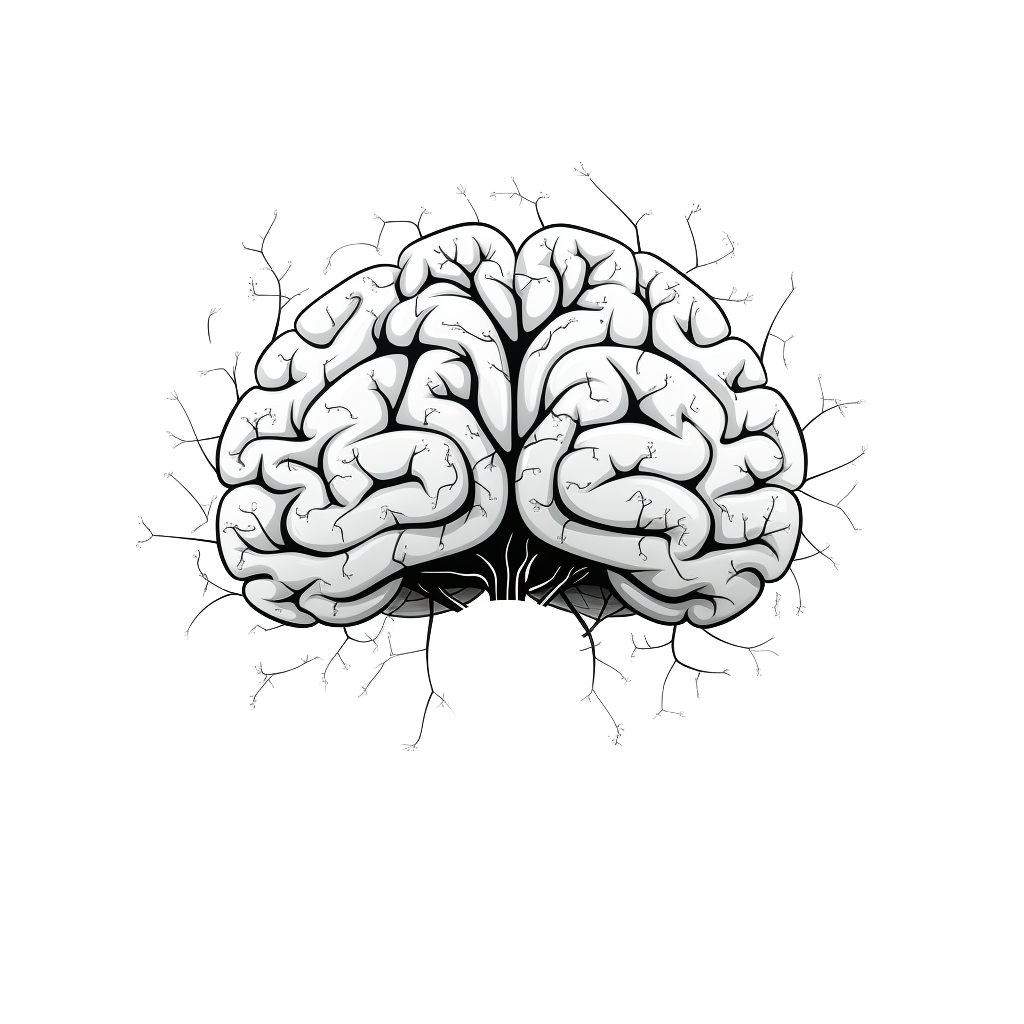
\includegraphics[width=.45\textwidth]{contents/01-introduction/figs/01-fep-brain.png}};
  \node[inner sep=0pt, opacity=0.25] (planet)[left=of center, xshift=3.5mm]{
\includegraphics[width=.45\textwidth]{contents/01-introduction/figs/01-fep-planet.png}};

  \node[box, minimum width=30mm, minimum height=10mm, fill=white](hidden)[left=of center, xshift=-10mm]{Hidden states};
  \node[box, minimum width=30mm, minimum height=10mm, fill=white](model)[right=of center, xshift=10mm]{Internal model};
  \node[box, minimum width=30mm, minimum height=10mm](sensory)[above=of center]{Sensory input};
  \node[box, minimum width=30mm, minimum height=10mm](actions)[below=of center]{Actions};

   \path[line, thick] (hidden) edge[out=90,in=180] node [] {} (sensory);
   \path[line, thick] (sensory) edge[out=0,in=90] node [] {} (model);
   \path[line, thick] (model) edge[out=270,in=0] node [] {} (actions);
   \path[line, thick] (actions) edge[out=180,in=270] node [] {} (hidden);

   \path[line, thick] (model) edge[out=180,in=270] node [] {} (sensory);
   \path[line, thick] (hidden) edge[out=0,in=90] node [] {} (actions);
   \path[line, thick, <->] (sensory) edge[out=270,in=90] node [] {} (actions);

\end{tikzpicture}}
  \caption{Schematic illustration of the reciprocal exchanges between an agent (on the right) and its environment (on the left).
    The hidden states of the environment are inferred using approximate posterior estimates within
    an internal model, which is conditioned on the activity of the agent's sensory receptors
    (sensory states).
    The internal states also infer the evolution of the agent's actuators (action states),
    enabling the agent to bring changes in the external states that align with the expected
    sensory states.
    The \acl{fep} states that the inference process in the internal model minimizes
    the \acl{vfe} in that model.
  }
  \label{fig:intro:fep}
\end{figure}

The concept that self-organizing biological systems, such as cells or brains, can be explained by their tendency to minimize \ac{vfe} is rooted in Helmholtz's work on unconscious inference \citep{helmholtz66, meyering_helmholtzs_1989} and has been further explored in psychology \citep{gregory_perceptions_1980} and machine learning \citep{dayan_helmholtz_1995}. 
Crucially, from an information processing viewpoint, \ac{vfe} minimization is the \textit{only}
ongoing process, and it is therefore responsible for all thought processes, learning,
decision-making, and ultimately, intelligent behavior.
In short, according to FEP, \textbf{the brain is a probabilistic model for sensory observations, and Bayesian inference in that model is the underlying process for natural intelligence}.

\subsection{Intelligent agents and the Active Inference framework}

\Ac{aif} is a corollary of \ac{fep} and describes how
natural agents might use \ac{vfe} minimization to infer potential future events and their next actions, in addition to the environmental causes of observations at the present time \citep{smith_step-by-step_2021, de_vries_factor_2017}.
If \ac{vfe} minimization in natural agents is responsible for intelligent reasoning and
decision making, the question arises if we can transfer these ideas to engineering and
consider the development of synthetic \ac{aif} agents that go out into the world and learn
purposeful behavior on-the-fly, without the need for a large training data set or reliance on
a power-hungry cluster of \acp{gpu}. And if we can, where should we start?

In fact, toy-sized \ac{aif} agents have already been designed and shown to work in practice
\citep{friston_active_2016,pio-lopez_active_2016,da_costa_active_2020,van_de_laar_active_2022, koudahl_realising_2023, van_de_laar_realising_2023},
however, the application of \ac{aif} for large-scale real-world problems remains a challenge.
The brain's exceptional computational capabilities for \ac{vfe} minimization include automated,
simultaneous (parallel), spontaneous (reactive), large-scale (billions of synapses),
time-varying processing of high-dimensional sensory data streams, in real time, under
ultra-low power (<20W) resource constraints.
Furthermore, the brain has the ability to adapt beliefs about environmental causes
(represented by model states) of new observations, update beliefs about model
parameters, and update the model structure over time under the pressure of minimizing
\ac{vfe}.

Sadly, there is no ``\ac{ai} software toolbox'' today that aims to support nature-inspired
intelligent agents solely through \ac{vfe} minimization, which makes it difficult to test these hypotheses in ``the field''. 
Motivated by \ac{fep}, this thesis is driven by the challenge of creating a practical software tool for Bayesian inference, 
where all processing stems from efficient \ac{vfe} minimization.
It is important to recognize that this work does not aim to provide a definitive solution to the complex problem of how intelligent synthetic agents should behave, learn, and be simulated. Instead, the goal is to take significant steps toward achieving these objectives. By exploring the principles and mechanisms proposed by \ac{fep} and \ac{aif}, this research contributes to the ongoing efforts of the research community and lays the foundation for further advancements.
% and eventually enabling the realization of synthetic \ac{aif} agents.